\documentclass[tikz,border=10pt]{standalone}
\usepackage{mathabx}
\usepackage{stackengine}
\usetikzlibrary{backgrounds}
\usepackage{newunicodechar}
\newunicodechar{♮}{$\natural$}
\newunicodechar{♭}{$\flat$}
\newunicodechar{♯}{$\sharp$}
\newunicodechar{➚}{$\nearrow$}
\newunicodechar{➘}{$\searrow$}
\newunicodechar{ʼ}{'}
\newunicodechar{Ả}{\stackon[0.8pt]{A}{,}}
\newunicodechar{Ɓ}{\stackon[0.8pt]{B}{,}}
\newunicodechar{Ƈ}{\stackon[0.8pt]{C}{,}}
\newunicodechar{Ɗ}{\stackon[0.8pt]{D}{,}}
\newunicodechar{Ẻ}{\stackon[0.8pt]{E}{,}}
\newunicodechar{Ƒ}{\stackon[0.8pt]{F}{,}}
\newunicodechar{Ɠ}{\stackon[0.8pt]{G}{,}}
\newunicodechar{Ȧ}{\stackon[0.8pt]{A}{.}}
\newunicodechar{Ḃ}{\stackon[0.8pt]{B}{.}}
\newunicodechar{Ċ}{\stackon[0.8pt]{C}{.}}
\newunicodechar{Ḋ}{\stackon[0.8pt]{D}{.}}
\newunicodechar{Ė}{\stackon[0.8pt]{E}{.}}
\newunicodechar{Ḟ}{\stackon[0.8pt]{F}{.}}
\newunicodechar{Ġ}{\stackon[0.8pt]{G}{.}}


\def\centerarc[#1](#2)(#3:#4:#5);%
{
  \draw[#1]([shift=(#3:#5)]#2) arc (#3:#4:#5);
}


\begin{document}
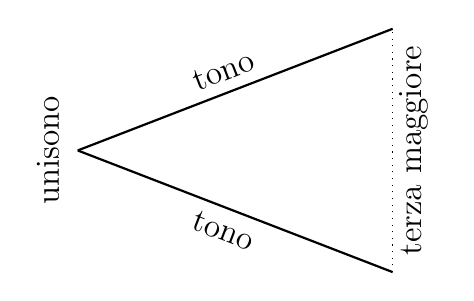
\begin{tikzpicture}

\draw[thick] (0.0,0.0) -- (4.0,-1.5452089);
\node[align=center] at (1.9063091, -1.0151371) { \rotatebox{-21.12165756125379}{\large tono} };
\draw[thick] (0.0,0.0) -- (4.0,1.5452088);
\node[align=center] at (1.9063091, 1.015137) { \rotatebox{21.121655132742088}{\large tono} };
\draw[dotted] (0.0,0.0) -- (0.0,0.0);
\node[align=center] at (-0.32000002, 0.0) { \rotatebox{90.0}{\large unisono} };
\draw[dotted] (4.0,-1.5452089) -- (4.0,1.5452057);
\node[align=center] at (4.32, -0.0000016212464) { \rotatebox{90.0}{\large terza maggiore} };
\end{tikzpicture}
\end{document}